\documentclass[11pt]{beamer}
\usetheme{CambridgeUS}
\usepackage[utf8]{inputenc}
\usepackage{amsmath}
\usepackage{amsfonts}
\usepackage{amssymb}
\usepackage[
backend=biber,
style=alphabetic,
citestyle=authoryear
]{biblatex}
\usepackage{array}
\usepackage{xcolor}

% Footnote without number
\newcommand\blfootnote[1]{%
  \begingroup
  \renewcommand\thefootnote{}\footnote{#1}%
  \addtocounter{footnote}{-1}%
  \endgroup
}
\def\boxit#1{%
  \smash{\color{red}\fboxrule=1pt\relax\fboxsep=2pt\relax%
  \llap{\rlap{\fbox{\vphantom{0}\makebox[#1]{}}}~}}\ignorespaces
}
\addbibresource{stats.bib}
\title[Bioestatística II] %optional
{Teste t de amostras independentes}

\subtitle{CGF2046 - Bioestatística II}

\author[da Silva, Ricardo] % (optional, for multiple authors)
{R. ~R. ~da Silva\inst{1}}

\institute[FCFRP] % (optional)
{
  \inst{1}%
  Departamento de Ciências BioMoleculares\\
  Faculdade de Ciências Farmacêuticas

}

\date{\today} % (optional)

\titlegraphic{
\includegraphics[width=5.8cm]{figs/logo_final}} 

\begin{document}

%\begin{frame}
%\titlepage
%\end{frame}

%\begin{frame}
%\tableofcontents
%\end{frame}

\begin{frame}
\titlepage
\end{frame}

\begin{frame}
\label{contents}
\frametitle{Sumário}
\tableofcontents
\end{frame}

\setbeamercovered{transparent}
\begin{frame}
\frametitle{Objetivos de Aprendizado\footcite{carlson2017introduction}}
  Depois de assitir essa aula e fazer as atividades complementares, você será capaz de:
  \\~\\
  \begin{itemize}
  \uncover<1->{\item
    Explicar quando usar um teste t de amostras independentes;}
  \uncover<2->{\item
    Explicar a lógica do teste t de amostras independentes;}
   \uncover<3->{\item
    Escrever hipóteses nulas e de pesquisa usando símbolos e palavras para testes unicaudais e bicaudais;}
   \uncover<4->{\item
    alcular graus de liberdade e definir uma região crítica para testes unicaudais e bicaudais;}
   \uncover<5->{\item
    Calcular amostras independentes t usando \textit{software};}
   \uncover<7->{\item
    Calcular e interpretar um tamanho de efeito (d);}
   \uncover<8->{\item
    Resumir os resultados da análise.}            
  \end{itemize}
\end{frame}

\section{Introdução ao teste t}
\setbeamercovered{transparent}
\begin{frame}
\frametitle{Amostras Independentes}
Até agora, você aprendeu a usar dois testes t diferentes: 

\begin{itemize}
\item \textit{t de amostra única}: usa-se sempre que quiser comparar uma média amostral com uma média populacional;
\item \textit{teste t de amostras relacionadas}: usa-se ao comparar as médias amostrais dos mesmos indivíduos medidos em dois momentos diferentes ou de pares de pessoas pareadas medidas sob condições diferentes.
\end{itemize}
Quando você precisar comparar duas médias amostrais que não estão relacionadas, você deve usar um terceiro teste t: \textit{um teste t de amostras independentes}.

\end{frame}

\setbeamercovered{transparent}
\begin{frame}
\frametitle{Amostras Independentes}
Por exemplo, suponha que você esteja interessado no efeito de um medicamento na perda de peso. Poderíamos pensae em três cenários:
\begin{itemize}
\item \textit{t de amostra única}: administrá-lo a uma amostra de pessoas e, depois de tomarem o medicamento por 1 mês, comparar a média de quilos perdidos pela amostra com zero quilos;
\item \textit{t de amostras relacionado}: medir o peso médio da amostra antes de tomar o medicamento e novamente um mês depois de tomar o medicamento;
\item \textit{teste t de amostras independentes}: administrar o medicamento a uma amostra de pessoas e um placebo a outra amostra.
\end{itemize}
\end{frame}

\setbeamercovered{transparent}
\begin{frame}
\frametitle{Fórmula conceitural para t de amostras independentes}
O teste t de amostras independentes é a razão entre a diferença média observada e a diferença esperada devido ao erro de amostragem:\\~\\

t = Diferença média das amostras - Diferença média esperada das populações se H0 for verdadeira/Diferença média esperada devido ao erro de amostragem\\~\\

O numerador é simplesmente a diferença entre as duas médias amostrais. O termo no denominador representa a quantidade de erro amostral esperado.

\[t = \frac{\bar{x}_1-\bar{x}_2}{SEM_i}\]

\end{frame}

\setbeamercovered{transparent}
\begin{frame}
\frametitle{Teste t de Amostras Independentes bicaudal}

\textbf{Exemplo:} Um pesquisador quer testar como os rótulos verbais influenciam a memória das imagens dos participantes. 
 
\begin{itemize}
\item Mostrar a todos os participantes uma série de 25 desenhos de linhas simples, e pedir-lhes que lembrem dos desenhos 10 minutos depois;
\item Metade dos participantes viu apenas os desenhos, enquanto a outra metade também viu uma descrição verbal de cada desenho semelhante;
\item Comparar a memória daqueles que viram os desenhos e as descrições verbais (isto é, o grupo experimental) com a memória daqueles que apenas viram os desenhos (isto é, o grupo de controle).
\end{itemize}

Optamos por um teste bilateral. Também escolhemos um \(\alpha=0.05\).

Grupo 1: Grupo com descrições verbais:
21, 22, 20, 20, 18, 20

Grupo 2: Grupo sem Descrições Verbais:
19, 20, 19, 18, 16, 20

\end{frame}

\setbeamercovered{transparent}
\begin{frame}
\frametitle{Rótulos verbais influenciam a memória das imagens?}

\begin{center}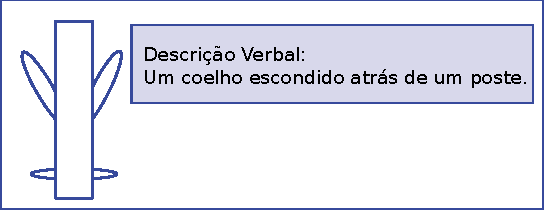
\includegraphics[width=0.9\linewidth]{figs/fig10.1} \end{center}

\end{frame}

\setbeamercovered{transparent}
\begin{frame}
\frametitle{Teste t de Amostras Independentes}

\begin{center}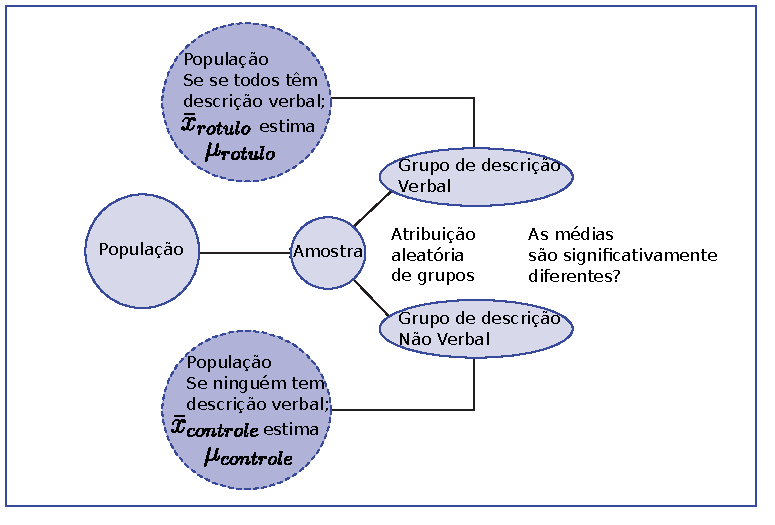
\includegraphics[width=0.9\linewidth]{figs/fig10.2} \end{center}

\end{frame}


\setbeamercovered{transparent}
\begin{frame}
\frametitle{Etapa 1: examinar as pressuposições estatísticas}

Todos os testes de hipóteses são baseados em suposições específicas e, se essas suposições forem violadas, esses testes podem produzir resultados enganosos.\\~\\
Os quatro pressupostos básicos são:

\begin{enumerate}
\item independência dos dados;
\item medição apropriada das variáveis para análise;
\item normalidade das distribuições;
\item homogeneidade da variância.
\end{enumerate}

\end{frame}

\setbeamercovered{transparent}
\begin{frame}
\frametitle{Etapa 1: examinar as pressuposições estatísticas}

Os quatro pressupostos básicos são:

\begin{enumerate}
\item \textbf{independência dos dados:} A VI presença ou ausência de descrições verbais, identifica dois grupos/condições diferentes;
\item \textbf{medição apropriada:} variável independente (VI) \(\Rightarrow\) identifica presença ou ausência de descrições verbais, variável dependente (VD) \(\Rightarrow\) número de desenhos de linhas lembrados corretamente, é medido em como uma variável quantitativa;
\item \textbf{normalidade das distribuições:} as distribuições das pontuações de memória tendem a ter formato normal e, portanto, essa suposição provavelmente é atendida;
\item \textbf{homogeneidade da variância:} utilizamos a regra geral de que se o desvio padrão numa condição for o dobro do de outra condição, esta suposição pode ser violada.
\end{enumerate}

Existem duas maneiras de calcular o erro de amostragem para um teste t de amostras independentes. Uma forma pressupõe homogeneidade de variância e a outra não. É possível utilizar testes, como o teste de Levene para determinar a homogeneidade das variância.

\end{frame}

\setbeamercovered{transparent}
\begin{frame}
\frametitle{Etapa 2: expor as hipóteses nulas e de pesquisa simbolicamente e verbalmente}

O teste t de amostras independentes determina se a diferença das média é significativamente diferente de 0.

\begin{center}
\begin{tabular}{ m{2cm}|m{3cm}|m{2cm}|m{3cm} } 
 \hline
 Tipo de Hipótese & Simbólico & Vebal & Diferença entre médias amostral e populacional\\
  \hline
 Hipótese nula & $H_0:\mu_1=\mu_2;$ ou & Diferença da médias $\approx$ 0 & Erro amostral \\
 & $H_0:\mu_1-\mu_2=0;$ & &\\
 Hipótese de pesquisa & $H_a:\mu_1 \neq \mu_2$ ou & Diferenças médias $\neq$ 0 & Descrição verbal afeta memória  \\ 
  & $H_a:\mu_1-\mu_2\neq0;$ & &\\
 \hline
 \hline
\end{tabular}
\end{center}

\end{frame}

\begin{frame}
\frametitle{Etapa 3: Use o tamanho da amostra para calcular os graus de liberdade e defina as regiões críticas}
A fórmula do gl para teste t de amostras independente é $gl = (n_1 - 1) + (n_2 - 1)$, onde $n_1$ e $n_2$ representam os tamanhos amostrais das duas amostras, espectivamente.

Neste caso, o gl é o seguinte:

\[gl = (n_1-1) + (n_2-1) = (6-1) + (6-1) = 10\]

\begin{columns}
\begin{column}{0.5\textwidth}
   Excerto da tabela t bilateral\\~\\

\begin{center}
\begin{tabular}{ccc} 
 \hline
gl & $\alpha = .05$ & $\alpha = .01$\\
9 &	2.262200 &	3.249800\\
\boxit{1.7in} 10 &	2.228100 &	3.169300\\
11 &	2.201000 &	3.105800\\
 \hline
\end{tabular}
\end{center}   
   
   
\end{column}
\begin{column}{0.5\textwidth}  %%<--- here
   \begin{itemize}
   \item O valor de corte de \(\alpha= .05\) define a região crítica, os valores t são improváveis se o valor nulo for verdadeiro.
   \end{itemize}
\end{column}
\end{columns}
\end{frame}

\setbeamercovered{transparent}
\begin{frame}
\frametitle{Etapa 4: calcular a estatística do teste (teste t de amostras relacionadas)}
\textit{4a. Calcule o desvio entre as duas médias amostrais}\\~\\

Existem dois termos no numerador da estatística t. A primeira $(\bar{x}_1 - \bar{x}_2)$ é a diferença entre as duas médias amostrais. O segundo $(\mu_1 - \mu_2)$ é a diferença entre as duas populações, assumindo que a hipótese nula é verdadeira. Assim, o numerador é simplesmente a diferença observada entre as duas médias amostrais:

\[(\bar{x}_1 - \bar{x}_2) = ( 20.17 - 18.67) = 1.50\]

\end{frame}

\setbeamercovered{transparent}
\begin{frame}
\frametitle{Etapa 4: calcular a estatística do teste (teste t de amostras relacionadas)}
4b. Calcule o erro de amostragem esperado
\[SQ_1 = \frac{1}{N-1}\sum_{i=1}^n(x_{1i} - \bar{x}_1)^2 = 1.767\]
\[DP_1 = \sqrt{1.767} = 1.329\]
\[SQ_2 = \frac{1}{N-1}\sum_{i=1}^n(x_{1i} - \bar{x}_1)^2 = 2.267\]
\[DP_2 = \sqrt{2.267} = 1.506\]

\end{frame}

\setbeamercovered{transparent}
\begin{frame}
\frametitle{Etapa 4: calcular a estatística do teste (teste t de amostras relacionadas)}
4b. Calcule o erro de amostragem esperado\\~\\
Quando apropriado, agrupar as variações tornará seu teste de significância mais preciso. A fórmula para a variância agrupada é a seguinte:

\[SQ_p = \frac{(n_1-1)SQ_1+(n_2-1)SQ_2}{(n_1-1)+(n_2-1)} = \frac{(6-1)1.767+(6-1)2.267}{(6-1)+(6-1)}=2.02\]
O método de cálculo do erro amostral que assume a homogeneidade da variância utiliza a variância agrupada para determinar o erro padrão estimado da diferença média ($SEM_i$)

\[SEM_i = \sqrt{\frac{SD_p}{n_1}+\frac{SD_p}{n_2}} = \sqrt{\frac{2.02}{6}+\frac{2.02}{6}} = 0.82\]

\end{frame}

\setbeamercovered{transparent}
\begin{frame}
\frametitle{Etapa 4: calcular a estatística do teste (teste t de amostras relacionadas)}

\textit{4c. Calcule a estatística do teste (teste t independente)}\\~\\

O teste t de amostras independente é a razão entre o desvio observado entre as duas médias amostrais dividido pelo erro padrão estimado da diferença média:

\[t = \frac{\bar{x}_1-\bar{x}_2}{SEM_i} =  \frac{20.17 - 18.67}{0.82} = 1.83\]

O valor t obtido não é suficientemente grande para rejeitar a hipótese nula e, portanto, você não rejeita a hipótese nula.
%\begin{center}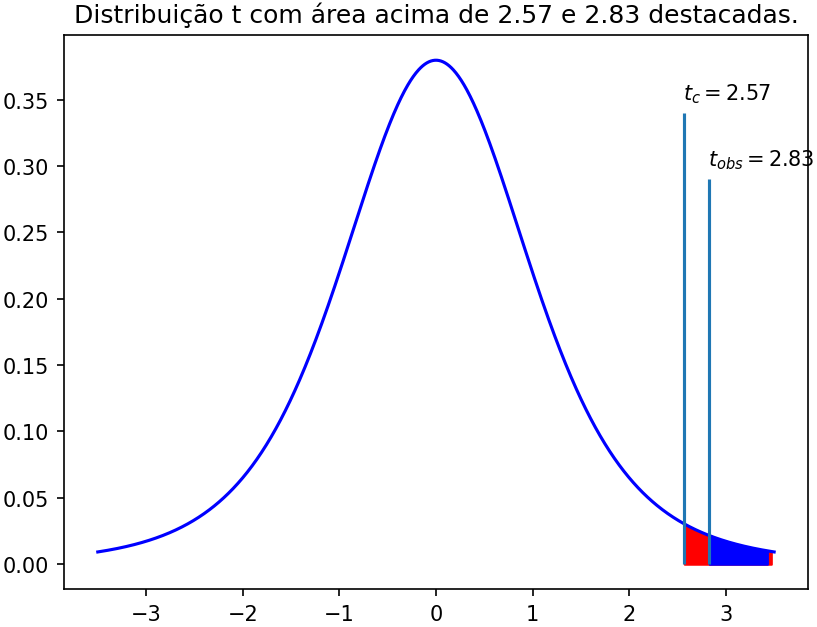
\includegraphics[width=0.55\linewidth]{figs/regiao_critica_observada_t_rel} \end{center}

\end{frame}


\setbeamercovered{transparent}
\begin{frame}
\frametitle{Etapa 5: calcule o tamanho do efeito e descreva se o seu grau}
A fórmula para calcular o tamanho do efeito de um teste t independente é semelhante à de um teste t de amostra única. No entanto, ao calcular d, o denominador é a variância combinada. 
\begin{align*}
d = \frac{\bar{x}_1 - \bar{x}_2}{SQ_p} = \frac{20.17-18.67}{2.02} = 1.06
\end{align*}
Quando a hipótese nula não é rejeitada e ainda assim houve um tamanho de efeito médio ou grande, o tamanho da amostra utilizado no estudo pode ter sido pequeno para que o teste estatístico ou o tamanho do efeito sejam confiáveis. Ao interpretar os resultados de qualquer estudo, também é importante considerar os resultados de outros estudos semelhantes.

\end{frame}

\setbeamercovered{transparent}
\begin{frame}
\frametitle{Etapa 5: calcule o tamanho do efeito e descreva se o seu grau}
A melhor maneira de interpretar qualquer tamanho de efeito é compará-lo com os tamanhos de efeito produzidos por estudos semelhantes na literatura de pesquisa. Se você não conseguir encontrar estudos semelhantes na literatura para fornecer uma referência, poderá usar as diretrizes gerais sugeridas por Cohen (1992) para interpretar os tamanhos dos efeitos na Tabela 6.2.

\begin{center}
\begin{tabular}{cc} 
 \hline
d  & Tamanho estimado do efeito\\
 \hline
Perto de 0.2 & Pequeno \\
Perto de 0.5 & Médio \\
Perto de 0.8 & Grande \\
 \hline
\end{tabular}
\end{center}   

\end{frame}

\setbeamercovered{transparent}
\begin{frame}
\frametitle{Etapa 6: Interpretando os Resultados do Teste de Hipóteses}

O parágrafo a seguir resume os resultados desses testes:\\~\\
Não houve diferença significativa entre as pontuações de memória daqueles que obtiveram as descrições verbais $(\bar{x}_1 = 20.17, DP_1 = 1.33)$ e daqueles que não obtiveram $(\bar{x}_2 = 18.67, DP_2 = 1.51)$, $t_{(10)} = 1.83$, $p > 0.05$, d = 1.06. No entanto, é importante notar que os tamanhos amostrais eram pequenos, portanto este estudo deve ser repetido com tamanhos amostrais maiores antes de serem tiradas conclusões.
\end{frame}

\begin{frame}
\frametitle{Exemplo de teste t de amostras relacionadas (unicaudal)}
\textbf{Exemplo:} Um psiquiatra recruta seis pessoas com altos índices de ansiedade para um estudo de avaliação do novo medicamento. Todos os seis voluntários completam um inventário de ansiedade antes de tomar o medicamento e novamente após tomar o medicamento por 1 mês.\\~\\ 

Espera-se que diminua os índices de ansiedade das pessoas que o tomam.
\end{frame}

\setbeamercovered{transparent}
\begin{frame}
\frametitle{Etapa 1: examinar as pressuposições estatísticas}

Todos os testes de hipóteses são baseados em suposições específicas e, se essas suposições forem violadas, esses testes podem produzir resultados enganosos.\\~\\
Os quatro pressupostos básicos são:

\begin{enumerate}
\item independência dos dados;
\item medição apropriada das variáveis para análise;
\item normalidade das distribuições.
\end{enumerate}

\end{frame}

\setbeamercovered{transparent}
\begin{frame}
\frametitle{Etapa 1: examinar as pressuposições estatísticas}

Os três pressupostos básicos são:

\begin{enumerate}
\item \textbf{independência dos dados:} A VI neste estudo identifica dois grupos relacionados, ou seja, antes vs. depois de tomar o medicamento;
\item \textbf{medição apropriada:} variável independente (VI) \(\Rightarrow\) identifica as duas condições de medicamento versus placebo, variável dependente (VD) \(\Rightarrow\) nível de ansiedade dos participantes, é medido em como uma variável quantitativa;
\item \textbf{normalidade das distribuições:} população original de diferenças médias é normalmente distribuida.
\end{enumerate}

\end{frame}

\setbeamercovered{transparent}
\begin{frame}
\frametitle{Etapa 2: expor as hipóteses nulas e de pesquisa simbolicamente e verbalmente}

O teste t de amostras relacionadas determina se a média dessas diferenças é significativamente menor do que 0.

\begin{center}
\begin{tabular}{ m{2cm}|m{2cm}|m{3cm}|m{3cm} } 
 \hline
 Tipo de Hipótese & Simbólico & Vebal & Diferença entre médias amostral e populacional\\
  \hline
 Hipótese nula & $\mu_{D}=0;$ & Diferença média $\approx$ 0 & Erro amostral \\ 
 Hipótese de pesquisa & $\mu_{D} < 0.$ & Diferença média $<$ 0 & Medicamento diminui ansiedade  \\ 
 \hline
 \hline
\end{tabular}
\end{center}

\end{frame}

\begin{frame}
\frametitle{Etapa 3: Use o tamanho da amostra para calcular os graus de liberdade e defina as regiões críticas}
Depois de saber o tamanho da amostra de um estudo, você precisa calcular seus graus de liberdade (gl). Para o teste t de amostra única, a fórmula para o gl é \textit{gl = N - 1}. Portanto, neste caso,
\[gl = 6 - 1 = 5\]

\begin{columns}
\begin{column}{0.5\textwidth}
   Excerto da tabela t unilateral\\~\\

\begin{center}
\begin{tabular}{ccc} 
 \hline
gl & $\alpha = .05$ & $\alpha = .01$\\
4 &	2.131800 & 3.746900\\
\boxit{1.7in} 5 & 2.015000 & 3.364900\\
6 & 1.943200 & 3.142700\\
 \hline
\end{tabular}
\end{center}   
   
   
\end{column}
\begin{column}{0.5\textwidth}  %%<--- here
   \begin{itemize}
   \item O valor de corte de \(\alpha= .05\) define a região crítica, os valores t são improváveis se o valor nulo for verdadeiro.
   \end{itemize}
\end{column}
\end{columns}
\end{frame}

\setbeamercovered{transparent}
\begin{frame}
\frametitle{Etapa 4: calcular a estatística do teste (teste t de amostras relacionadas)}
\textit{4a. Calcule D para cada participante/par correspondente}\\~\\

A primeira etapa no cálculo da estatística t das amostras relacionadas é calcular o valor da diferença (ou seja, D) para cada par de valores. 

\begin{center}
\begin{tabular}{cccc} 
 \hline
Voluntário & Antes & Depois & D (Depois - Antes)\\
 \hline
A & 22 & 19 & -3\\
B & 22 & 19 & -3\\
C & 23 & 18 & -5\\
D & 26 & 25 & -1\\
E & 23 & 20 & -3\\
F & 25 & 21 & -4\\
 \hline
\end{tabular}
\end{center}   

\end{frame}

\setbeamercovered{transparent}
\begin{frame}
\frametitle{Etapa 4: calcular a estatística do teste (teste t de amostras relacionadas)}
\begin{itemize}
\item 4b. Calcule a diferença média observada ($\bar{x}_D$)

\[\bar{x}_D = \frac{\sum_{i=1}^n D_i}{N} = \frac{-19}{6} = -3.167\]

\item 4c. Calcule a diferença média esperada devido ao erro de amostragem
\[QM_D = \frac{1}{N-1}\sum_{i=1}^n(D_i - \bar{x}_D)^2 = 1.77\]
\[SEM_D = \frac{DP}{\sqrt{N}} = \frac{1.329}{\sqrt{6}} = 0.543\]
\item 4d. Calcule a estatística do teste (teste t de amostras relacionadas)
\[t =  \frac{\bar{x}_D}{SEM_D}  = \frac{-3.167}{0.543} = -5.83\]
\end{itemize}
\end{frame}

\setbeamercovered{transparent}
\begin{frame}
\frametitle{Etapa 5: calcule o tamanho do efeito e descreva se o seu grau}
Um tamanho de efeito é um índice da diferença entre a média da amostra e a média da população. A estatística de tamanho do efeito normalmente usada ao comparar duas médias é d. 
\begin{align*}
d &= \frac{Desvio\quad observado\quad entre\quad as\quad medias}{Desvio\quad padrao}\\
  &= \frac{\bar{x}_D}{DP_D} = \frac{-3.167}{1.329} =  -2.38
\end{align*}

\end{frame}


\setbeamercovered{transparent}
\begin{frame}
\frametitle{Etapa 6: Interpretando os Resultados do Teste de Hipóteses}

As frases a seguir resumem os resultados deste estudo:\\~\\

As pessoas apresentaram níveis de ansiedade mais baixos (\(\bar{x}_D = 20.33\), DP = 2.50) depois de tomar o medicamento do que antes de tomar o medicamento (\(\bar{x}_D = 23.50\), DP = 1.64), \(t_{(5)} = -5.83\), \(p < 0.05\) (unicaudal), d = -2.38. A redução nos valores de ansiedade foi bastante grande, mais de 2 desvios padrão. O tamanho da amostra neste estudo foi muito pequeno. Um estudo mais amplo deve ser feito antes de se tirar qualquer conclusão sobre o medicamento.

\end{frame}


\setbeamercovered{transparent}
\begin{frame}
\frametitle{Exemplo 9.1}
Uma distribuidora de combustíveis deseja verificar se um novo tipo de gasolina é eficaz na revitalização de motores velhos. Com esse objetivo, seleciona 12 automóveis de um mesmo modelo com mais de 8 anos de uso e, após regulagem de seus motores, verifica o consumo de combustível. Em seguida o carro é abastecido com o novo tipo de combustível durante 15 semanas, e uma nova aferição do consumo é feita. O novo combustível é eficaz na melhora do rendimento? Conclua com \(\alpha=0.05\).

\begin{table}[h]
\tiny
\centering
\begin{tabular}{|c|c|c|c|c|c|c|c|c|c|c|c|c|}
\hline
Autom. & 1 & 2 & 3 & 4 & 5 & 6 & 7 & 8 & 9 & 10 & 11 & 12 \\
\hline
Após (Y) & 11.6 & 8.8 & 9.9 & 9.5 & 11.6 & 9.1 & 10.6 & 10.8 & 13.4 & 10.6 & 10.5 & 11.4 \\
\hline
Antes (X) & 8.1 & 7.9 & 6.8 & 7.8 & 7.6 & 7.9 & 5.7 & 8.4 & 8.0 & 9.5 & 8.0 & 6.8 \\
\hline
D = Y-X & 3.5 & 0.9 & 3.1 & 1.7 & 4.0 & 1.2 & 4.9 & 2.4 & 5.4 & 1.1 & 2.5 & 4.6 \\
\hline
\end{tabular}
\end{table}

\end{frame}

\setbeamercovered{transparent}
\begin{frame}
\frametitle{Referências bibliográficas}
\printbibliography
\end{frame}

\end{document}